\chapter{Quasiparticle Interference (QPI)}
%todo: to write the abstract of this chapter after finishing this chapter
%todo: to standardize the vector form in this chapter 

\section{Introduction to Quasiparticle}
Quasiparticle is any long-lived, well-defined excitation in a system that behaves like a particle, it is a semi-classical term used to describe particle interactions in terms of renormalized single-particle excitation. In Fermionic systems, it correspond to a sharp peak in the spectra function: 
	\[
	A(\mathbf{k}, \omega) = -\frac{1}{\pi} \frac{\operatorname{Im} \Sigma(\mathbf{k}, \omega)}{(\omega - \tilde{E}_{\mathbf{k}})^2 + [\operatorname{Im} \Sigma(\mathbf{k}, \omega)]^2},
	\]
%todo: cite Landau's original paper
%the development of quasiparticle theroies has a long history going back all the way to 1940s and 50s during the investigation of quantum liquids \textsuperscript{3}He and \textsuperscript{4}He. 

The development of quasiparticle model for Fermionic system started in 1940s, when Sommerfeld and Bethe\cite{SommerfeldBethe1933} developed a model for non-interacting electron gas, also known as the 'Fermi gas', in which a series of important terms are introduced. Consider a system made of non-interacting electrons with momentum $k$ and spin $\sigma = 1/2$, and is in touch with an electron reservoir with chemical potential $\mu$. The occupation number naturally follows the Fermi-Dirac distribution $n_{k,\sigma}=1/(1+e^{(k^2/(2m)-\mu)/T}))$. At $T=0$, the occupation thus has a sharp boundary famously known as the Fermi surface, in the momentum space confined by the Fermi wave number $k_f$, and the energy defined by the Fermi surface is called the Fermi energy. At non-zero temperature, electrons at the Fermi energy will started to be excited to above the Fermi energy, this excitation can also be described in second-quantization by the creation of a quasiparticle with energy: $\epsilon_{k,sigma} = k^2/2m - \mu$. 

Sommerfeld's theory of electron gas worked quite well in normal metallic systems, but the success is unexpected, as the model neglected the Coulomb interaction between electrons. In a metallic system where the electron separation is in the order of lattice spacing, the Coulomb interaction is in the order of eV, which is much larger than other, say the thermal excitation considered in the electron gas mode. 

In late 1960s, Landau raised a theory of Fermi liquid with a series of foundational papers\cite{Landau1956}\cite{Landau1957}, to address that even in the presence of interactions, we can find fermionic excitations in these many-body systems, and describe these excitations with what is known as the Landau quasiparticles. By adding a time variant interaction term, defined by time constant $\zeta$ to the non-interactive system, and constructing the system Hamiltonian as
\begin{equation}\label{adiabatic}
	H_{\zeta} = H_0 + H_{\text{int}} e^{-\zeta t}, \quad t > 0,
\end{equation}

By the principle of adiabatic continuity, Landau is able to bridge between the states of interactive and non-interactive system. The consequence is that the states describing interactive system can now be reduced to states in the non-interactive system with the same quantum numbers $k, \sigma$. More specifically, as quoted from \textit{What is a Quasi-Particle?} by J.R.Schrieffer, "these many-body states are well characterized in terms of a set of elementary excitations, called quasi-particles, which for the interacting system play the same role as the excited electrons(above the Fermi surface) and the excited holes(below the Fermi surface) in the Independent-particle approximation(IPA)". 

Landau's quasiparticle is an extremely useful concept in computing the screening and the transport properties of an electron-gas-like system. However, we should emphasis that the theory is only valid with several assumptions:

For adiabatic procedure to hold, time scale $\zeta$ in \ref{adiabatic} should be bounded by two conditions: 1. rate of evolution should be small compared to the energy of the state: $\zeta << \epsilon_{k,\sigma}$, 2. the final bound state remains the same as the initial one, meaning the lifetime $\tau_{life}$ of the bound state should be long enough: $\tau_{life} >> \zeta^{-1}$. Therefore, $\zeta$ should suits: 
\begin{equation}
	\tau_{life}^{-1} << \zeta << \epsilon_{k,\sigma},
\end{equation}
since typical excited energy is in the order of temperature, and the lifetime is inversely proportional to $T^2$, we can also write:
\begin{equation}
	T^2 << \zeta << k_B T,
\end{equation}
This requirement can be satisfied at a range of low temperature. Later we will also see that the requirements also extend to the energy level of the states, as the quasiparticle lifetime decreases as the energy deviate from the Fermi energy. 
%todo: can refer to the chapter where we talk about the lifetime decay with simulation. 
Therefore, Landau's theory of Fermi liquid postulated that an interacting fermionic system can we mapped adiabatically to a non-interacting Fermi gas, with long-lived quasiparticle that shares the same quantum numbers near the Fermi surface. It works in a regime with weak to moderate correlations at sufficiently low temperatures, and thus why worked extremely well in explaining properties in simple and noble metals. For more detailed reading regarding the theory, the textbooks of Pines and Nozieres\cite{nozieresTheoryQuantumLiquids2018a} Nozieres \cite{nozieresDerivationLandauTheory1962} offers derivations and in depth discussions. 

Landau's theory failed to address more involved systems, however, based on the theory, scientists managed to formulate a more generalized concept of quasiparticle through the lens of Green's function scheme of many-body perturbation theory, here I would like to provide a rought list of the theories chronologically that extended or refined quasiparticle to new regimes:
\begin{itemize}
	\item\textbf{Hatree-Fock Approximation (HF)} (1930s)
	HF approximation is not an extension of Fermi liquid theory but it is the first step beyond a purely free-electron model, and it lays groundwork for diagrammatic expansions \cite{fockNaeherungsmethodeZurLoesung1930}, \cite{slaterNoteHartreesMethod1930}.
	
	\item\textbf{Random Phase Approximation(RPA)} (1950s): 
	RPA extend the theory to moderate correlations where long-range screening is crucial, included dynamical screening. Successfully explains plasmon dispersion and optical properties in metals and semiconductors \cite{bohmCollectiveDescriptionElectron1951}, \cite{nozieresCorrelationEnergyFree1958}.
	
	\item\textbf{GW Approximation} (1965)
	GW approximation provided a more accurate approximation than RPA and can be implemented to stronger correlated systems \cite{hedinNewMethodCalculating1965}, \cite{aryasetiawanGWMethod1998}.
	
	\item\textbf{Dynamical Mean-Field Theory(DMFT)} (1990s)
	DMFT was developed via a non-perturbative approach, this allows it to extend the concept of quasiparticles to account for strong local correlations in systems like transition metal oxides and f-electron materials. Although it kept the concpt of quasiparticles, it showed that they failed near Mott transitions when electron-electron interaction is large enough \cite{metznerCorrelatedLatticeFermions1989}, \cite{georgesDynamicalMeanfieldTheory1996}.
	
	\item\textbf{GW + DMFT} (2000s)
	This combined method took the best of GW(dynamic and non-local screening) with DMFT(local, but exact correlation), making it suitable for systems with moderate to strong correlation as well as significant screening effects, like heavy fermion compounds \cite{biermannFirstprinciplesApproachElectronic2003}.
\end{itemize}


\section{Introduction to Quasiparticle Interference measurement}

\subsection{Terminology}
To set stage for the discussion in this chapter, we must make distinctions between the following terminologies: 
\begin{itemize}
	\item \ac{QPI}: a physical phenomenon describing the interference of all possible quasiparticles, a concept used to describe the collective behavior of a group of particles. examples of quasiparticle excitation include phonon in crystalline solids, Bogoliubov quasiparticle in superconductors etc. 
	\item QPI pattern: a pattern that can be observed in different physical system that corresponds to the physical phenomenon QPI.
	\item QPI measurement: a measurement that measures the QPI patterns presented in systems that intrinsically host QPI.
\end{itemize}
We should note that STM is not the only tool that can perform QPI measurement. In fact, interference of quasiparticles are reported across a wide literature in different systems using different techniques. For example,
%todo: to wirte different examples here, template as X used Y technique to detect G quasiparticle Interference pattern in Z system.: ranging from crystalline excitation like phonon in Si phononic crystals \cite{maldovan_phonon_2015}, electronic excitation like Bogoliubov quasiparticle in superconductors interference strongly\cite{homan_search_nodate}

I will then elaborate what these terms mean in the context of STM study, and to reduce redundancy, in the following writing, QPI, QPI pattern and QPI measurement will be referred specifically to STM studies.

\subsection{what is QPI measurement in STM studies}
%todo: to plot a standard grid and its FFT here.
In a word. QPI measurement is an STM technique that aims to probe the band structure of a material by studying QPI patterns presented on the surface of a material. 

Imagine an ideal metal with no crystal imperfection, with Landau's Fermi liquid theory, we know that the Landau quasiparticle has an eigenstate described by a Bloch wavefunction: 

\begin{equation}
\psi(\mathbf{r}) = e^{i \mathbf{k} \cdot \mathbf{r}} u(\mathbf{r})
\label{eq:bloch}
\end{equation} 
where $k$ is the crystal momentum of the quasiparticle. And the electron \ac{LDOS} can be written as  
\begin{equation}
\text{LDOS}(E, \vec{r}) \propto \sum_k |\Psi_k(\vec{r})|^2 \delta(E - \varepsilon(k))
\label{eq:ldos}
\end{equation}

where  $\epsilon(k)$ is the energy dispersion of the Bloch state for different $\vec{k}$. And if we plug Equation (\ref{eq:bloch}) into Equation (\ref{eq:ldos}), we see that $\text{LDOS}$ is translationally invariant at all Bravais-lattice-equivalent points. Thus why in ideal case, real space imaging technique like \ac{STM}, can not be used to measure $\epsilon(k)$. 

However, crystal imperfections as discussed in Ch.4 can help us introduce a momentum texture to the $\text{LDOS}(E, \vec{r})$. In low temperature STM, where the phonon modes and other excitation are rare or absent, lattice imperfections such as point defects can cause elastic scattering which mixes electronic eigenstates at different $\vec{k}$ but at the same energy, the interference between the incoming and outgoing wave forms a "standing wave" that act as a real space modulation in $\text{LDOS}(E)$ described as a impurity-induced Friedel oscillation\cite{benaFriedelOscillationsDecoding2016}. This spatial modulation in $\text{LDOS}$ is the QPI pattern that we refer to in STM studies. We can perform \ac{STS} measurement on the region that presents this QPI pattern, then perform Fourier transformation to the STS, we can observe this QPI pattern in the momentum space. This whole process of detecting QPI pattern and analyze it in momentum space is what we call a QPI measurement. 

We will show case this \ac{LDOS} modulation with a simulation on a toy model in the following section. 

\begin{figure}
	\centering
	\includegraphics[width=0.5\textwidth]{example-image-a} % Replace with your image file
	\caption{Friedel oscillation and QPI}
	\label{fig:example}
\end{figure}

\subsection{LDOS modulation simulation on a square lattice}

As mentioned in last section \ac{QPI} measurement is the Fourier transformed spatial \ac{STS} measurement, which is proportional to the \ac{LDOS}. Thus, to understand \ac{QPI} measurement, we must understand the origin of \ac{QPI} pattern and how it modifies \ac{LDOS}. Here, I present an investigation into the \ac{LDOS} modulation caused by point defects on a square lattice, this textbook exercise is inspired by work from Cheung et al \cite{cheungDictionaryLearningFouriertransform2020}.

\subsubsection{Theory}
We first consider a square lattice with lattice constant $a$, and model it through the single-electron \ac{TB} model considering only nearest-neighbor hopping. This hopping is characterized with a fixed negative number $t$ named hopping-parameter. We then place $N_d$ number of defects onto different lattice sites as a perturbation to the \ac{TB} Hamiltonian $H_0$. The total Hamiltonian can then be written as: 
$\hat{H} = \hat{H}_0 + \hat{H}_d$. $\hat{H}_d$ can be written as: 
\[
\hat{H}_d = \sum_{\alpha=1}^{N_d} E_\alpha \lvert \alpha \rangle \langle \alpha \rvert,
\] 
where $\alpha$ enumerates $\alpha^{th}$ defect located at $x_\alpha$, with energy $E_{\alpha}$ much smaller than hopping parameter $t$, we then write the \ac{TB} Hamiltonian and transfer it into momentum space:
\begin{align}
\hat{H}_0 = E_0 -t \sum_{j,\tau} (c_j^{+} c_{j+\tau} + c_{j+\tau}^{+} c_j) \label{h0_real} \\
\hat{H}_0 = E_0 -\sum_{k} \epsilon_k c_k^{+} c_k \label{h0_k} \\
\epsilon_k = -2t(cos(k_x a)+cos(k_y a)) \label{E_k}
\end{align}
Now we consider our measurable \ac{LDOS} $\rho(\mathbf{x},\omega)$:
\begin{equation}
\rho(\mathbf{x},\omega) = \rho^{0}(\mathbf{x},\omega) - \frac{1}{\pi} \operatorname{Im} \left[ \langle \mathbf{x} | \hat{G}_0 \hat{T} \hat{G}_0 |\mathbf{x} \rangle \right],
\label{ldos}
\end{equation}
where $\hat{G}_0$ and $\hat{T}$ are the \ac{BLGF} and the scattering T-matrix, respectively, according to the pertubative scattering theory. Since we are interested in the modulation of \ac{LDOS} caused by the defects, our actual observable is $\delta \rho(\mathbf{x}, \omega) \equiv \rho(\mathbf{x}, \omega) - \rho^{(0)}(\mathbf{x}, \omega)
$, which is the second term in Equation (\ref{ldos}).
To start, we need to compute the matrix element of \ac{BLGF} $G_0(\mathbf{x},\mathbf{x'},\omega)$:
\begin{align}
	G_0(\mathbf{x},\mathbf{x}';\omega) &= \langle \mathbf{x} | \hat{G}_0(\omega) | \mathbf{x}' \rangle, \\
\end{align}
where
\begin{align}
	\hat{G}_0(\omega) &= \int_{\text{BZ}} \mathrm{d}\mathbf{k} \, \frac{1}{\omega - \hat{H}_0} \lvert \mathbf{k} \rangle \langle \mathbf{k} \rvert \nonumber \\ 
	&= \int_{\text{BZ}} \mathrm{d}\mathbf{k} \, \frac{1}{\omega - E_\mathbf{k}} \lvert \mathbf{k} \rangle \langle \mathbf{k} \rvert,
\end{align}
where we have $\omega= \omega + i\epsilon$ to indicate the retarded green's function and to capture the analytic continuation. Then we remind ourselves that in 2D, $\langle \mathbf{k}|\mathbf{x} \rangle = (\frac{1}{\sqrt{2\pi}})^2 e^{-i\mathbf{k}\mathbf{x}}$, and plug the energy dispersion Equation (\ref{E_k}) in, we get: 
\begin{align}
	G_0(\mathbf{x}, \mathbf{x}') = 
	\frac{1}{(2\pi)^2} \frac{1}{2t} 
	\int_{\text{BZ}} \mathrm{d}\mathbf{k} \, 
	\frac{e^{i k_1 (x_1 - x_1')} e^{i k_2 (x_2 - x_2')}}{b + \left( \cos(k_1 a) + \cos(k_2 a) \right)}. 
\end{align}
where $b \equiv \frac{\omega+ i\epsilon-E_0}{2t}$ is a dimensionless parameter, to  we can then define a normalized position deviation $s_j \equiv \frac{1}{a}(x_j-x_j')$ and further reduced the matrix element to its final form: 
\begin{align}
	G_0(\mathbf{x}, \mathbf{x}') = 
	\frac{1}{(2\pi)^2} \frac{1}{2t a^2} 4 \, I_{\text{sq}} 
	\left( \frac{x_1 - x_1'}{a}, \frac{x_2 - x_2'}{a}, b \right) \label{blgf},
\end{align}
where
\begin{align}
	I_{\text{sq}}(s_1, s_2, b) \equiv 
	\int_0^\pi \int_0^\pi \mathrm{d}\phi_1 \, \mathrm{d}\phi_2 \, 
	\frac{\cos(s_1 \phi_1) \cos(s_2 \phi_2)}{b + \cos\phi_1 +b  \cos\phi_2} \label{Isq}.
\end{align}
Now we proceed to compute the matrix element of T-matrix, we know that: 
\begin{equation}
	\hat{T} = \hat{H_d} (\hat{I} - \hat{G_0}\hat{H_d})^{-1}.
\end{equation} 
And for locations $x_\alpha$, $x_\beta$ on defect sites $\alpha$ and $\beta$, we have: 
\begin{align}
	T_{\alpha\beta} &= \langle \alpha|\hat{H_d} (\hat{I} - \hat{G_0}\hat{H_d})^{-1} | \beta\rangle \\
	&= E_\alpha(\langle \alpha|\hat{I}|\beta\rangle - \langle \alpha|\hat{G_0}\hat{H_d}|\beta \rangle)^{-1} \\
	&= E_\alpha(\delta_{\alpha \beta} - E_\beta G_0(\mathbf{x_\alpha},\mathbf{x_\beta}))^{-1} \label{T_matrix_ele}.
\end{align}
Now with both matrix elements of the \ac{BLGF} and T-matrix, we can finally express $\delta\rho(\mathbf{x},\omega)$ as 
\begin{align}
	\delta\rho(\mathbf{x},\omega) &= - \frac{1}{\pi} \operatorname{Im} \left[ \langle \mathbf{x} | \hat{G}_0 \hat{T} \hat{G}_0 | \mathbf{x} \rangle \right] \\
	&= -\frac{1}{\pi} \operatorname{Im} \left[\sum_{\alpha, \beta=1}^{N_{\text{d}}} G_0(\mathbf{x}, \mathbf{x}_\alpha) T_{\alpha, \beta} G_0(\mathbf{x}_\beta, \mathbf{x})\right].
\end{align}
In single defect case, where $\mathbf{x_\alpha} = \mathbf{x_\beta} = \mathbf{x_d}$, we have: 
\begin{align}
	T(\mathbf{x_d},\omega) &= E_{\text{d}} \left( 1 - E_{\text{d}} G_0(\mathbf{x_d}, \mathbf{x_d}) \right)^{-1} \label{T_matrix_ele} \\
	&= \frac{1}{E_{\text{d}}^{-1} - G_0(\mathbf{x_d}, \mathbf{x_d}; \omega)},
\end{align}
and therefore: 
\begin{align}
	\delta\rho(\mathbf{x},\omega) &= - \frac{1}{\pi} \operatorname{Im}(\frac{G_0^2(\mathbf{x},\mathbf{x_d};\omega)}{E_d^{-1} - G_0(\mathbf{x_d},\mathbf{x_d};\omega)}) \label{singleldos}. 
\end{align}
And Equation (\ref{singleldos}) can be evaluated numerically with Equation (\ref{blgf}) and Equation (\ref{Isq}).

\subsubsection{Simulation result}
A repository for \ac{LDOS} simulation on the model described above is made and shared on this \hyperlink{https://github.com/Plswearpants/QPI_simulation}{github repository}

The setup of simulation is illustrated in \ref{fig:ch5_qpisim_demo}, a grid of $128x128$ in real space covering a $20x20$ lattice space indicated in orange dots. We can implant defects on different lattice sites, indicated in green dots. 

\begin{figure}
	\centering
	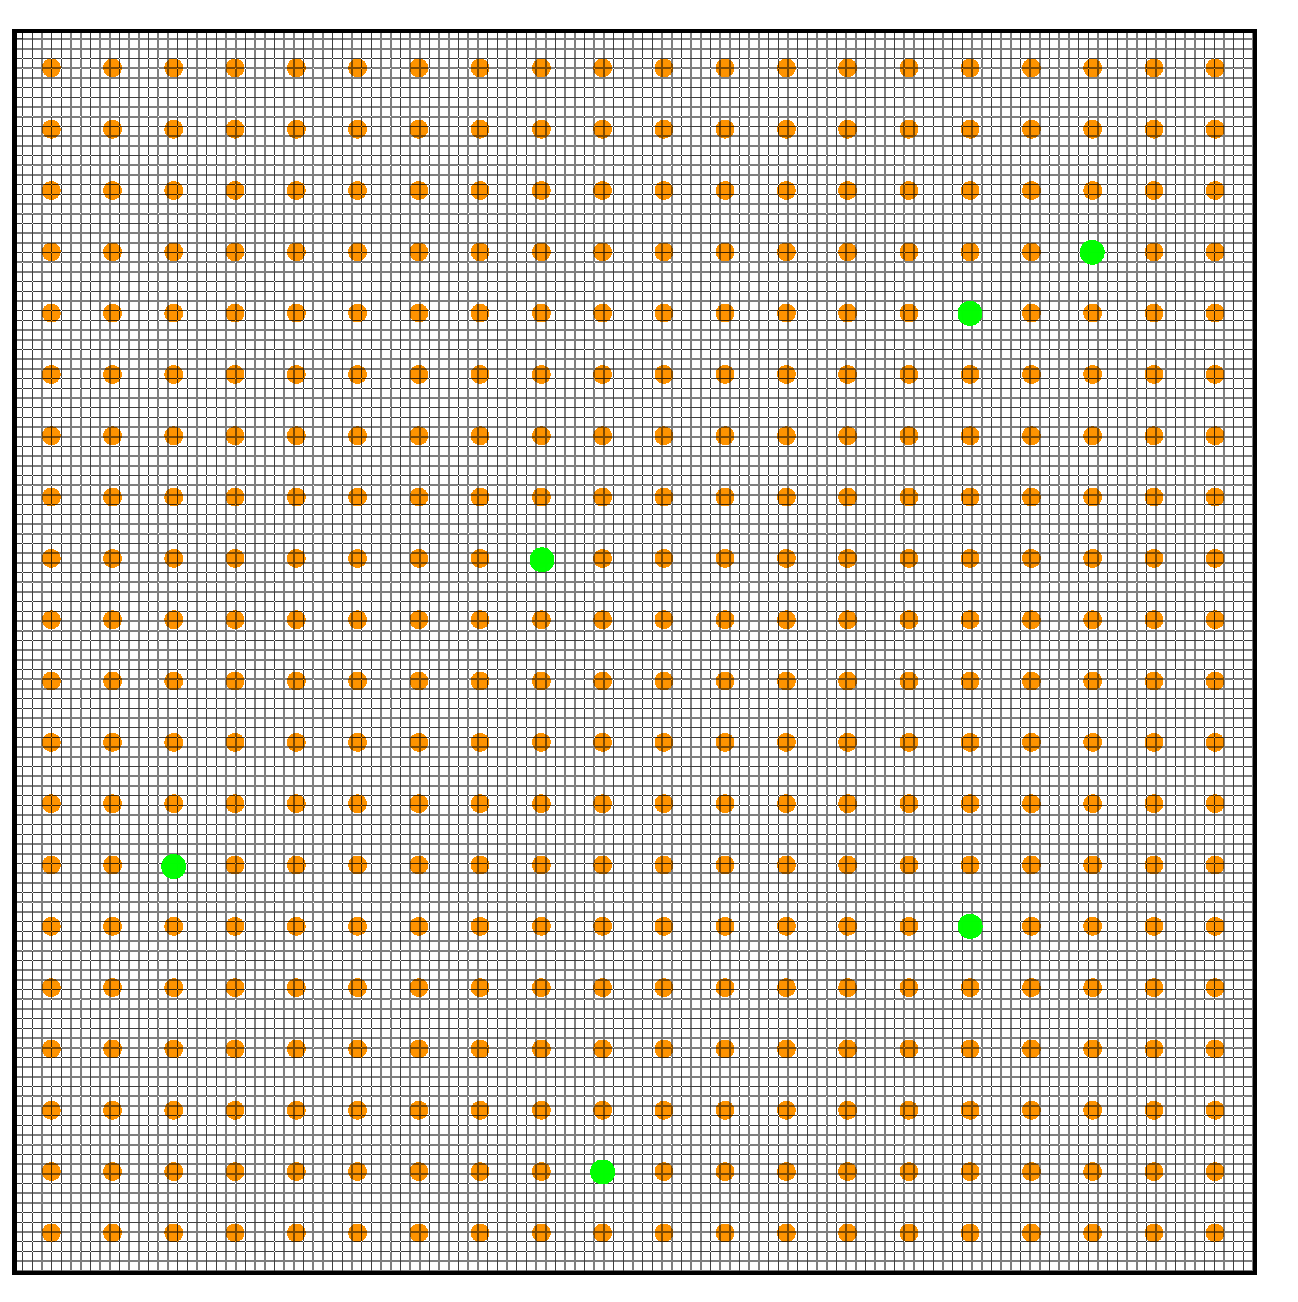
\includegraphics[width=\textwidth]{Ch5_QPIsim_demo.pdf}
	\caption{schematics for the simulation}
	\label{fig:ch5_qpisim_demo}
\end{figure}

A typical \ac{LDOS} map is shown in \ref{fig:ch5_single_scattering}, the image is cropped from a simulation where $\delta\rho$ was numerically computed at a $301x301$ grid chosen to overlap with the square lattice with $50x50$ sites, a single defect is placed on location $\mathbf{x_d}=0$, with defect energy $E_d$, hopping parameter $t$, onsite energy $E_0$, 41 energy slices are computed in an energy range of $(-0.5, 0.5)V$. 

Observations can be made on this simulation, in particular, we can see that:
1. The \ac{LDOS} modulation is featured by wave-like pattern similar to the Friedel oscillation we seen, and the pattern varies with energy.
2. The modulation is strongly correlated with the underlying lattice corrugation. 
3. Although the feature is decaying away from the defect location, the wave extend far into the space, indicating a relatively long life-time of this quasiparticle. And the life-time is especially long around the Fermi level.


\begin{figure}
	\centering
	\includegraphics[width=0.5\textwidth]{example-image-b} % Replace with your image file
	\caption{single defect scattering result, details: }
	\label{fig:ch5_single_scattering}
\end{figure}

\subsubsection{Single defect result}

\subsubsection{Multi defect result}
\begin{itemize}
	\item direct evaluation of $\delta\rho(\mathbf{x},\omega)$
	\item Convolution approach
\end{itemize} 
Estimating the multidefect result with convolution approach inherently makes assumption into the independent nature of scattering, which is only true for weak scattering and sparse impurity distributions. 

\subsubsection{Limitations and assumptions}


\subsubsection{the process}
\subsubsection{the result}


\section{Experimental QPI measurement}
Realspace \ac{QPI} signals are obtained by taking the grid map experiment on a region that presents \ac{QPI} patterns. In this section we will briefly explore \ac{QPI} measurement in the \ac{STM} experiment, more specifically, we will introduce the factors that dictate \ac{QPI} quality, discuss how to choose proper parameters that result in a good \ac{QPI} measurement, and finally we will present a specific challenge called the phase noise, which motivates our work in the next chapter.


\subsection{QPI measurement and quality}
As mentioned in Ch.2, taking a grid map is very involved. A successful grid map requires both an ideal instrumental setup and a set of proper measurement parameters based on the understanding of the targeting material. 

The key objective of an ideal instrumental setup is to create a stable environment and lower the system noise; as we discussed in Ch.2, this involves minimizing the noise from mechanical vibration, temperature fluctuation, and electronic instability of the system and maintaining a stable tip-surface tunneling junction. 

A grid map is defined by a $N\times N$ (assuming square) grid on a targeted area of $L \times L$ $nm^2$, this provides a spatial resolution $\Delta L = \frac{L}{N}$; In reciprocal space, this set up gives a range $Q = \frac{2 \pi}{\Delta L}$ with resolution $\Delta Q = \frac{2\pi}{L}$, the energy range and resolution is defined by the setting of the single-point spectroscopy performed on every grid point. 

A set of proper parameters for \ac{QPI} measurement aims to extract the most amount of information with the highest level of resolution given the constraints of the system. The most important constraint is the limiting cryogenic holding time. This puts a ceiling on the grid map run time, while different systems vary; typically, the cryogenic holding time is a fraction of a week. Within the boundary of the run time, we usually aim for a grid with a fine reciprocal resolution $\Delta Q$ and a reasonable reciprocal range $Q$, corresponding to a large field of view $L$ and a reasonable $\Delta L$. It is intuitive to have a proper size of reciprocal range $Q$ that is not infinitely large, as most of the q-space features reside within the Bragg peaks, exemplified by Fig. \ref{fig:ch5_ldos} c). But we also do not want the field of view $L$ to be too large, this is because in real experiments with finite noise level, the featured \ac{QPI} pattern has a finite lifetime and its intensity will dive under the noise at some cutoff distance $r_{cutoff}$ from the defect center; Thus, a field of view larger than the cutoff distance will instead decrease the signal to noise ratio. We illustrate cutoff distances in systems with different noise levels in Fig. \ref{fig:ch5_cutoff}. The noise level is set to be noiseless, SNR = 10, and SNR = 1.2, respectively; given the noise level shown in the green dotted line, we identify the furthest signal peak higher than the noise level and place a blue vertical line there. These vertical lines indicate the cutoff distances; and we can see with increasing noise level, $r_{cutoff}$ drops, and thus the optimal field of view should also drop.  

\begin{figure}
	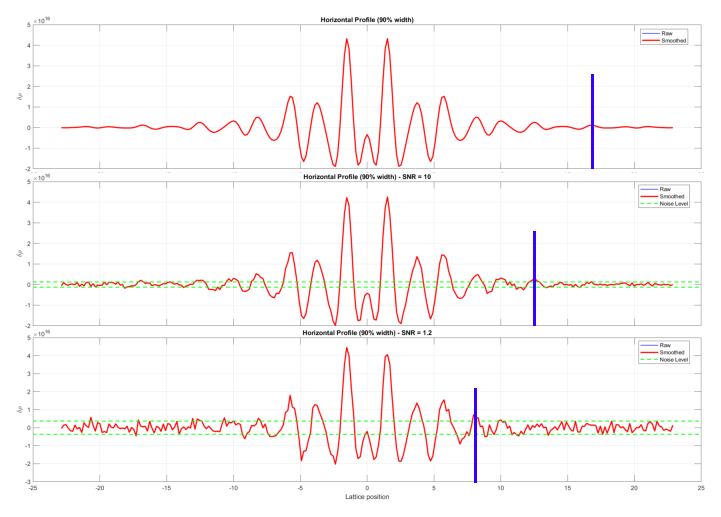
\includegraphics[width=\textwidth]{Ch5_fieldofview.pdf} 
	\centering
	\caption{Cutoff distances of QPI patterns with different signal-to-noise ratios. Three Horizontal Line profiles on $\delta\rho(\textbf{x}, E=0.45eV)$ with the noise of various levels. a) has no noise applied; b), c) have Gaussian noises applied with SNR = 10 and 1.2, respectively. Here the signal strength is defined as the variance of the noiseless $\delta\rho(\textbf{x}, E=0.45eV)$, see a) of Fig. \ref{fig:ch5_single_scattering}.}
	\label{fig:ch5_cutoff}
\end{figure}


\subsection{multi-defect QPI pattern and phase noise}
\ac{QPI} patterns present themselves around defects. While an ideal \ac{QPI} measurement is performed on isolated defects in a large field of view, it is normally difficult to find such a case. In real experiments, grid maps are usually taken on areas with multiple defects; this causes interference between the \ac{QPI} patterns originating from different defects, as hinted by Ch.5.2.4 when discussing Fig. \ref{fig:ch5_multi_scattering}.

This is problematic when we try to interpret the \textbf{q}-space \ac{QPI} map. As illustrated in Fig. \ref{fig:ch5_phasenoise}, when we have multiple defects scattered in the field of view, we start to see some noise patterns associated with the spatial distribution of the defects, as we can see by comparing c) and e), we see that with nothing but the relative locations of the defects changed, the corresponding \textbf{q}-space \ac{QPI} maps possess different noise patterns. This effect is called phase noise; it hinders our ability to analyze the underlying quasiparticle scattering process. 

\begin{figure}
	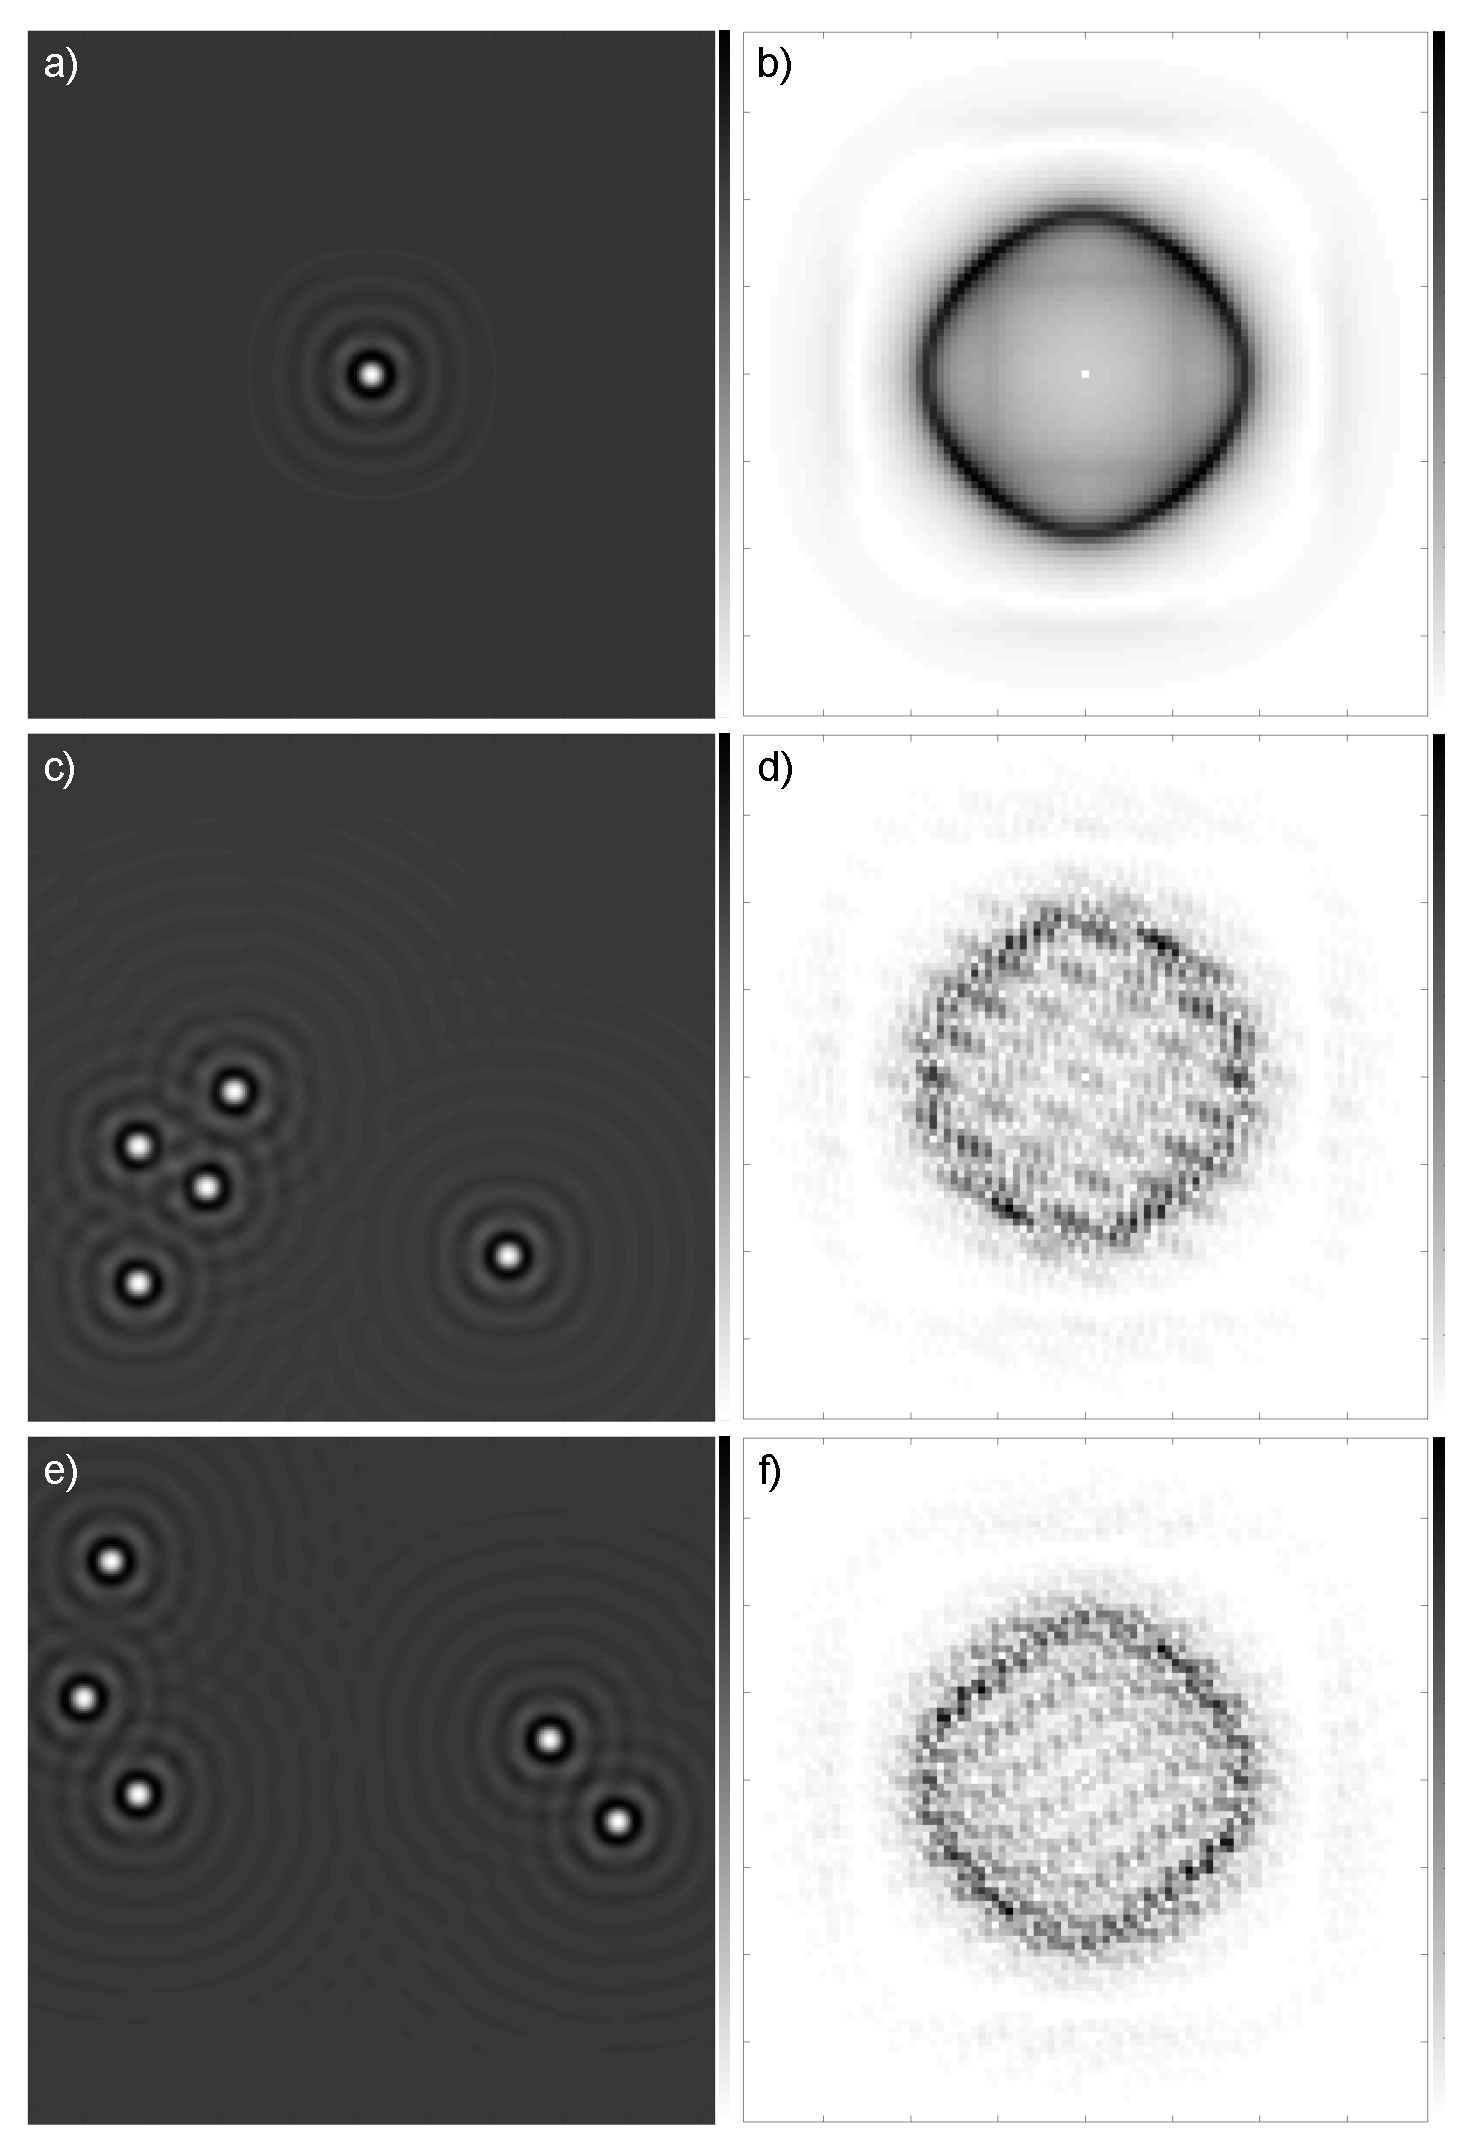
\includegraphics[width=0.85 \textwidth]{Ch5_phasenoise.pdf} 
	\centering
	\caption{Phase noise illustration. a),b): single defect scattering pattern and corresponding \textbf{q}-space QPI map. c)-f): multi-defect scattering with the same number of defects with different distributions, the corresponding QPI map presents phase noise with different patterns that associate with the defect distribution}
	\label{fig:ch5_phasenoise}
\end{figure}

Beyond the phenomenological illustration, we can further understand the source of phase noise with a mathematical analysis on multi-defect $\delta\rho(\textbf{x},\omega)$. We first discuss the form of the multi-defect T-matrix T, which is a $N_d \times N_d$ square matrix with entry T$_{\alpha \beta}$ representing the cross scattering term between defect m and n. We then separate the diagonal and off-diagonal terms and express T as\cite{leonard1972}:
\begin{align}
	\ T_{\alpha\beta} &= t_{\alpha} \delta_{\alpha\beta} + t_{\alpha} G_{0\alpha\beta} (1 - \delta_{\alpha\beta}) t_{\beta} + \sum_{\alpha' \neq \alpha, \beta} t_{\alpha} G_{0\alpha\alpha'} t_{\alpha'} G_{0\alpha'\beta} t_{\beta} + \cdots \label{eq_tmul}\\
	\label{eq.536}
	&= t_{\alpha} \delta_{\alpha\beta} + t_{\alpha} \sum_{\alpha'} \check{G}_{\alpha\alpha'} \ T_{\alpha'\beta},
\end{align}
\noindent where $t_{\alpha}$ is the T-matrix of a single impurity at site $\alpha$ and expressed on a matrix form in a localized basis set (i.e., expressed as the matrix with the same dimension as the multi-defect case but with only the $\alpha$'s diagonal entry none empty). And matrix $\check{G}_{\alpha\alpha'} = G_{0\alpha\alpha'}(1-\delta_{\alpha\alpha'})$, it contains the off-diagonal part of the Green's function. It has been shown by Fang et al. \cite{fangTheoryQuasiparticleInterference2013} that, in the Born approximation to the scattering amplitude, the first term dominates over the second term, and the latter can be omitted. We can, therefore, approximate multi-defect scattering with multiple single-defect scattering events. 

This approximation was then extended to the strong scattering case by Philipp et al. \cite{russmannInitioTheoryFourierTransformed2021}, under the assumption that the impurity concentration is low and the largest part of the surface is covered by pristine atoms and far from the impurities. They then utilized Equation \ref{eq.536} and further expressed the Green's function difference:

\[
\Delta G(\mathbf{r}, \mathbf{r}, E) = \int d^3 \mathbf{r}' \int d^3 \mathbf{r}'' \, G_0(\mathbf{r}, \mathbf{r}'; E) \, T(\mathbf{r}', \mathbf{r}''; E) \, G_0(\mathbf{r}'', \mathbf{r}; E)
\]

\begin{align}
	\label{eq.537}
	\Delta G_{\alpha \alpha} &= \Delta G^{(1)}_{\alpha \alpha} + \Delta G^{(2)}_{\alpha \alpha} \\
	\label{eq.538}
	&= \sum_{\alpha'} G_{0\alpha \alpha'} t G_{0\alpha' \alpha} + \sum_{\alpha'} G_{0\alpha \alpha'} t\sum_{\beta \beta'} \check{G}_{\alpha' \beta} \, T_{\beta \beta'} G_{0\beta' \alpha}.
\end{align}

\noindent By applying the stationary phase approximation \cite{lounisTheoryRealSpace2011} to $G_{0\beta'\alpha}$, and utilize the transnational symmetry of Bare lattice Green's function $G_0$, they showed:
\[
\Delta G^{(2)}_{\alpha\alpha}=\sum_{\alpha'}G_{0\alpha\alpha'}t\sum_{\beta\beta'}\check{G}_{\alpha'\beta}T_{\beta\beta'}K_{\beta'\alpha}e^{ik_{\beta'\alpha}\cdot R_{\beta'\alpha}},
\]
\noindent where the contribution of the last phase, $e^{ik_{\beta'\alpha}\cdot R_{\beta'\alpha}}$ can not be lifted, and is thus the source of the phase noise we observed in Fig. \ref{fig:ch5_phasenoise}. 

It is further noted that the contribution of the phase can be piratically canceled if we sum over all configurations of randomly distributed defects, which correspond to an infinitely large scanning surface, which can never be achieved. However, a decreased influence of this phase noise can be seen if we increase the density of the defects, as illustrated in Fig \ref{fig:ch5_changephasenoise}. This is because the patterns created by the phase noise become more fine-grained and can eventually be seen as featureless, similar to the random distribution of noise.  
%todo: verify whether this is true with more literature reviews. 

\begin{figure}
	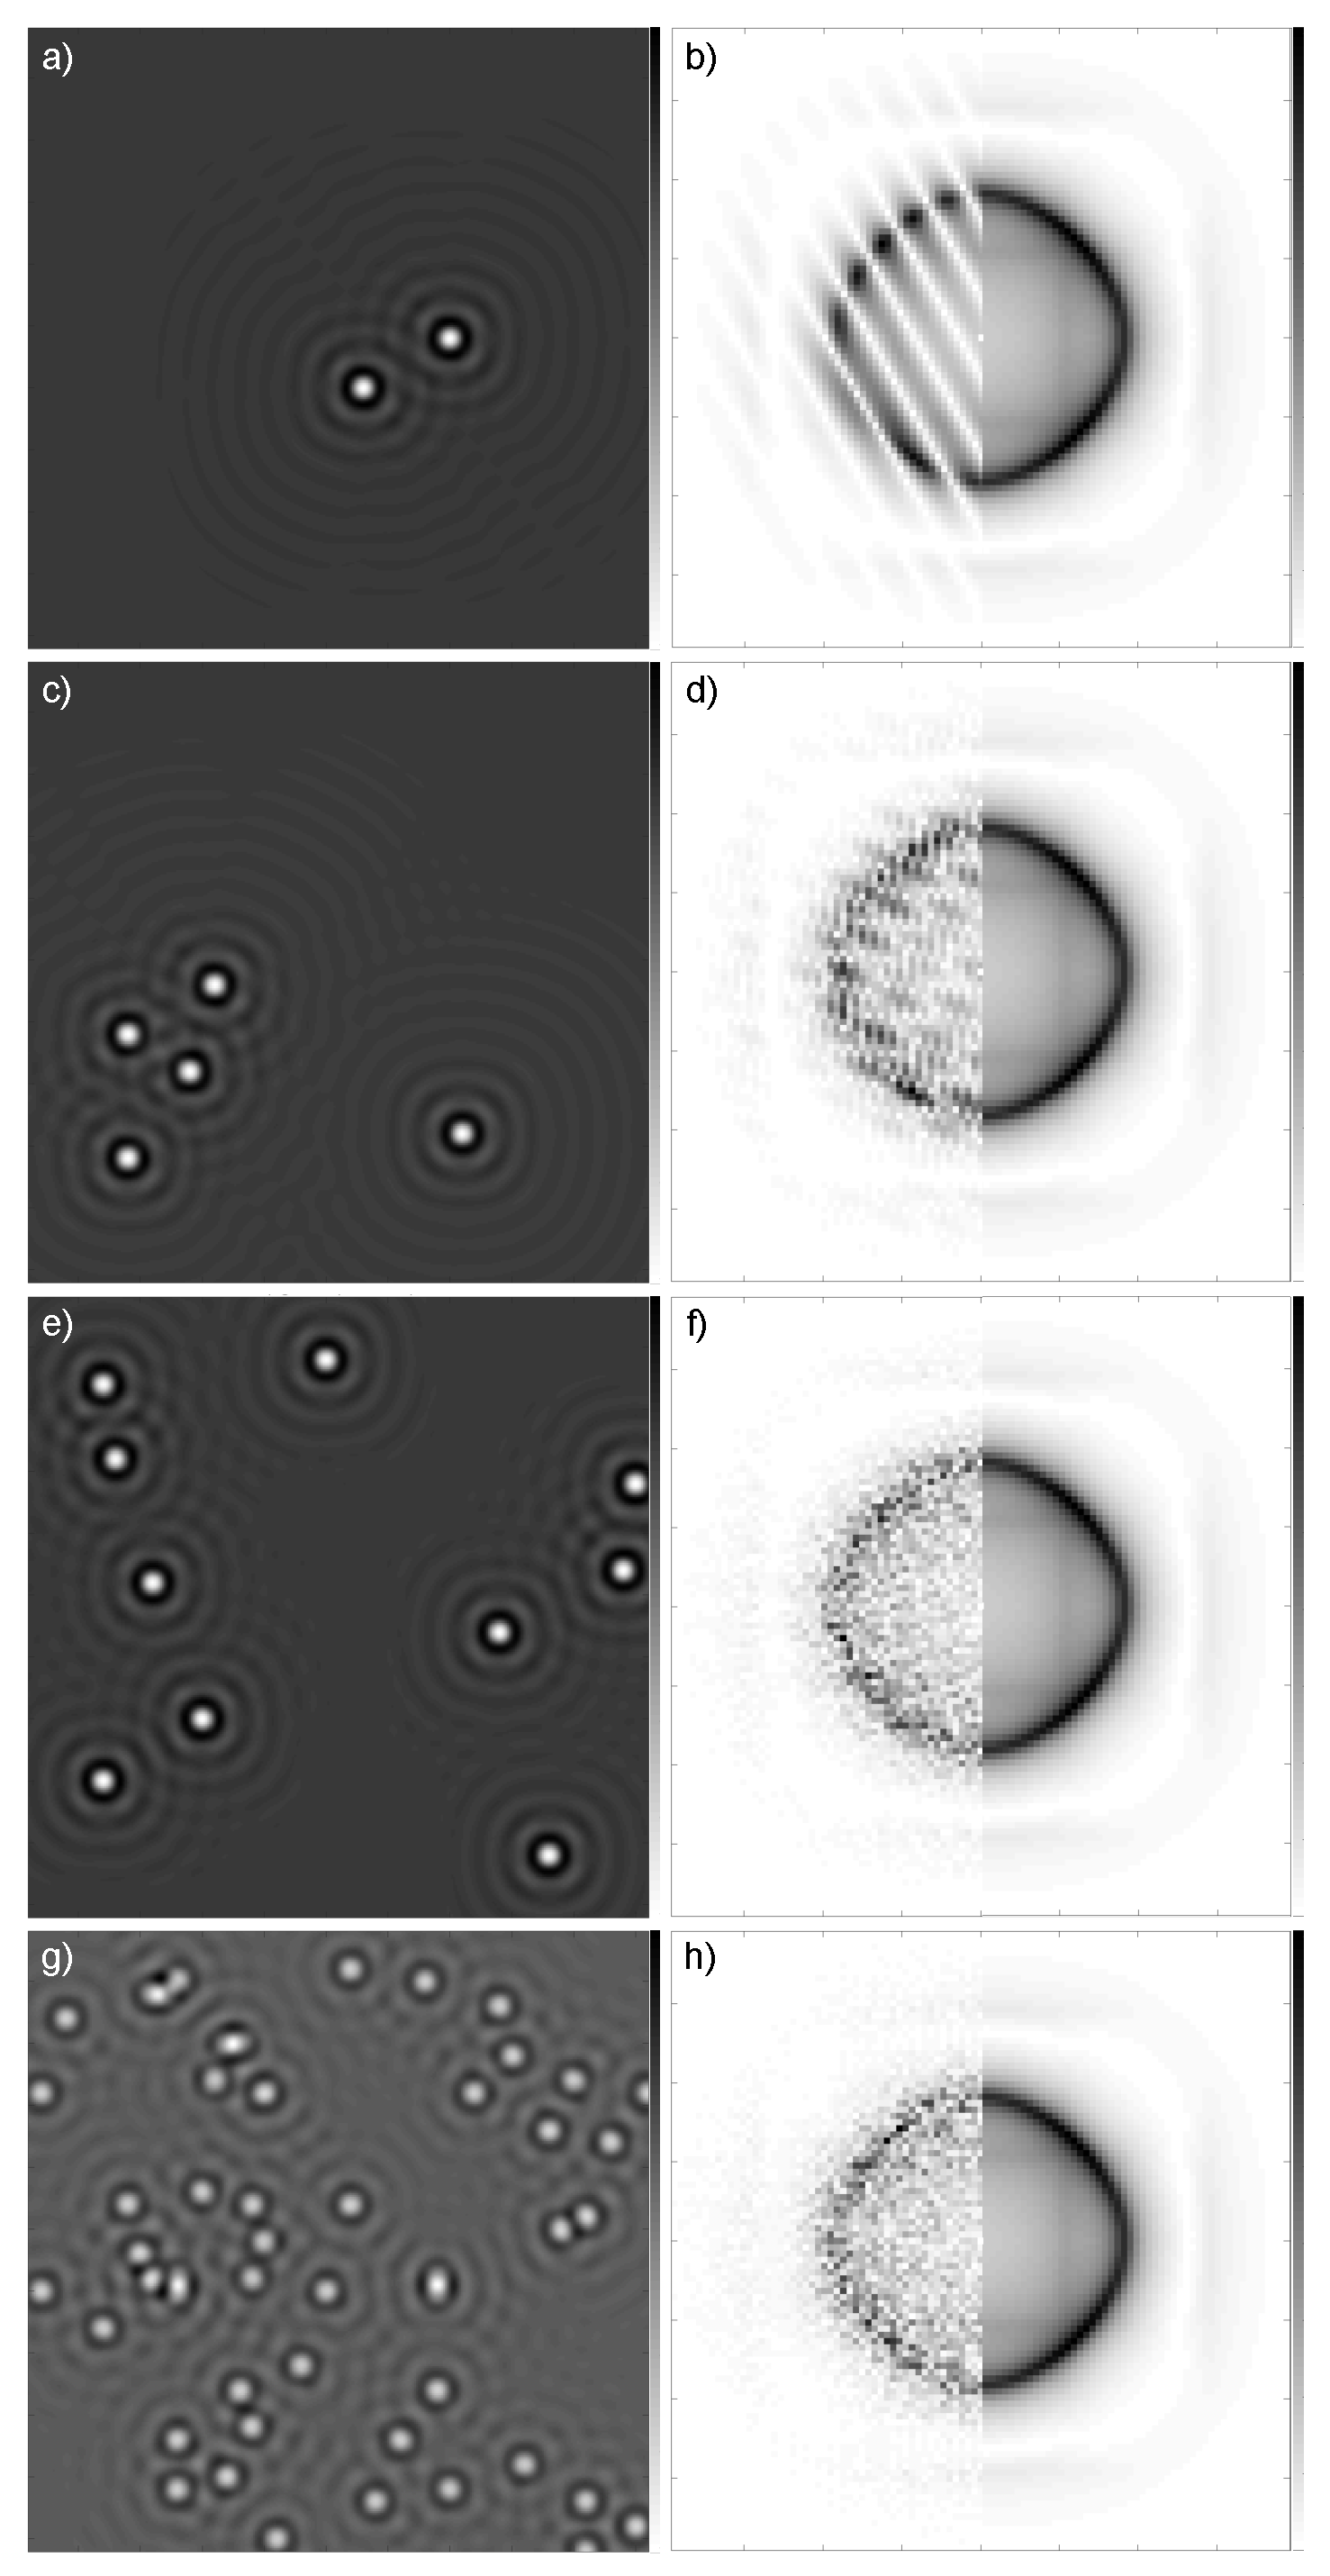
\includegraphics[width=0.7 \textwidth]{Ch5_changephasenoise.pdf} 
	\centering
	\caption{The effect of the phase noise is most prominent in the sparse defects regime. a)-h): $\delta\rho(\textbf{r},\omega)$ and \textbf{q}-space QPI plotted in pair with increasing defect concentration, showing the phase noise becomes more featureless. Single-defect QPI map is presented for reference on the right half of the \textbf{q}-space QPI.}
	\label{fig:ch5_changephasenoise}
\end{figure}
